%
% Niniejszy plik stanowi przykład formatowania pracy magisterskiej na
% Wydziale MIM UW.  Szkielet użytych poleceń można wykorzystywać do
% woli, np. formatujac wlasna prace.
%
% Zawartosc merytoryczna stanowi oryginalnosiagniecie
% naukowosciowe Marcina Wolinskiego.  Wszelkie prawa zastrzeżone.
%
% Copyright (c) 2001 by Marcin Woliński <M.Wolinski@gust.org.pl>
% Poprawki spowodowane zmianami przepisów - Marcin Szczuka, 1.10.2004
% Poprawki spowodowane zmianami przepisow i ujednolicenie 
% - Seweryn Karłowicz, 05.05.2006
% Dodanie wielu autorów i tłumaczenia na angielski - Kuba Pochrybniak, 29.11.2016

\documentclass[en]{pracamgr}

\autor{Mateusz Bajorek}{385122}

\title{Analysis and visualization of programmers’ activities during their workday}
\titlepl{Analiza i wizualizacja aktywności programistów w ramach ich dnia pracy}

\kierunek{Computer Science}

% Praca wykonana pod kierunkiem:
% (podać tytuł/stopień imię i nazwisko opiekuna
% Instytut
% ew. Wydział ew. Uczelnia (jeżeli nie MIM UW))
\opiekun{dr Robert Dąbrowski\\
  Institute of Informatics\\
  }

% miesiąc i~rok:
\date{September 2022}

%Podać dziedzinę wg klasyfikacji Socrates-Erasmus:
\dziedzina{11.3 Informatics, Computer Science}

%Klasyfikacja tematyczna wedlug AMS (matematyka) lub ACM (informatyka)
\klasyfikacja{D. Software}

% Słowa kluczowe:
\keywords{keystrokes dynamics}

% Used Latex packages
\usepackage{hyperref}
\usepackage{xcolor} % TODO TEMP!!!

% Tu jest dobre miejsce na Twoje własne makra i~środowiska:
\newtheorem{definition}{Definition}[section]

% koniec definicji

\begin{document}
\maketitle

\begin{abstract}
Similarly to another professions, programmers create their own working style. It can be characterized by
different phases of the day, splitting tasks into a few chunks, taking breaks, or focusing on a few
projects at the same time. In this thesis, I analyze if there exist links between programmers preferences
and the spectre of their duties for example, if it is true that front-end programmers work usually in the
evenings. For this purpose, I conduct a research scheme on a sample of programmers with the help of a self-created software tool for gathering anonymized data (including the number of projects, time of
activities, programming languages or particular frameworks usage). The end result of this thesis, are the
conclusions from the analysis of the aforementioned data with included visualizations. The tool used
in the thesis is shared publicly for the willing actors to independently verify my end results by
re-running the experiments or running new ones to gather new information for example about potential
improvements in programmers efficiency.
\end{abstract}

\chapter*{Acknowledgements}
\textcolor{red}{TODO}

First of all, I would like to thank my supervisor PhD Robert Dąbrowski for expert guidance during the "Software Optimization, Visualization and Analysis" (SOVA) seminars. His help in the university administrative procedures involving this thesis and overall assistance and patience in overcoming various obstacles was invaluable. 
% patience, many tips, critical insight

Another lecturer present during the seminars was Prof. Krzysztof Stencel who provided me with essential advice which I appreciate greatly. I also thank for his attempts at help in gathering the data for me.

Apart from the leaders of the seminars, I must mention my colleagues who were present at my presentations. This was the time when we shared our remarks on each other's work. My thesis would not be the same without their input during these discussions.

I especially thank (highlight from my colleagues) Małgorzata E. Z. Galińska (née Biegała) for testing and assistance with debugging of my addon.
% for being the first to test

My former employers and dear friends M. Asberg (CEO NewNative) and R. Dembkowski (CEO RadCode) for the help with gathering the data.
% and every employee who decided to share the data
% using their professional contacts and oportunities

I thank everyone who decided to share their data with me to proceed with my research project.

I am grateful for the Faculty of Mathematics, Mechanics and Informatics of the University of Warsaw for being able to study Computer Science and conduct my research there.

Lastly, my thanks go to my friends and family for their immense patience and unwavering support (also financial and emotional).

\begin{flushright}
Warsaw, December 2022

Mateusz Bajorek
\end{flushright}


\tableofcontents

\chapter{Introduction}

Programmers job focuses on developing computer software through all phases including design, testing and maintenance. These processes are executed according to the principles of performance, reliability and security \cite{Sto21ProgrammersDo}. With the industry maturing, upholding these rules in ever-expanding projects have become crucial to fulfill growing needs stated i.a. in software level agreements (SLAs). One of the answers to that have been the agile software development \cite{Gro21SDMHistory}, where actions like joining regularly scheduled team meetings, contacting clients or attending conferences have been universalized. Nevertheless, writing code has remained a key part of programmers job for the majority of them. In my study, I focus on analyzing and visualizing the exact process of writing software in an integrated development environment (IDE), largely omitting the other aforementioned aspects of being a programmer.

Research in the relevant areas differs depending on the context that is industrial or educational. Tracking of programmers time happens to be an essential part of the job in the IT industry. The reports provided by programmers are the basis for calculating a salary or even deciding the future of an employee by the management. For many programmers it may be hard to determine which activities constituted billing time or if different activities should be treated differently. In my own experience, hard to fix bugs or complicated issues solving which took many trials and errors happened to be particularly hard when it comes to calculating the exact amount of billing hours it took me and how to prove this reported effort to my employer. Those obstacles constituted my initial desire to explore the domain of programming process analysis and visualization. Nowadays there exist tools that measure the time automatically and compile the reports with almost no additional human effort.

In the industry there is less focus on the detailed analysis of the process of writing the code and more on the activities done during the whole workday. Process of writing the code is more of a concern for educational research and IDE development companies like JetBrains who want to know how users interact with their products and how to make them more ergonomic. In educational research people try to evaluate students based on their typing behavior. Apart from that, it's possible to authenticate users based on their typing characteristics.

% It was then I came up with researching this area a bit further. My idea was to track programmers activities even before they create any meaningful output. Of course, you could argue that the paradigms of continuous integration already solve this problem, however at the heart of my concerns lied the relatively high granularity of the data, which would be practically unachievable just by utilizing common paradigms (you do not imagine a programmer committing her/his work to git every minute or even more frequently without a high nosedive of her/his productivity).

The thesis contains 5 chapters and appendices. In the chapter \ref{r:background} there are studied basic concepts and related works both in analysis and in visualization techniques. The chapter \ref{ch:methodology} describes the tool used to gather and analyse the data. In the chapter \ref{ch:results} the results are presented and in the next one \ref{ch:discussion} they are discussed. The last two chapters conclude the whole thesis with suggestions for future work \ref{ch:conclusions} and provide links to the additional published materials \ref{ch:publishing}. I clarify that the pronoun “I” used in this thesis refers to its author.

% Say what it is about and what not. Say what data you use and which not. Say what to expect.

% Say that by activities you mostly mean just keystrokes.

% It's important to mention here that I am not interested in resources of data such as surveys, and only the factual data sources as there exists evidence that the programmers perception is inconsistent with the real data. Reference here.

% Mention that educational approaches can be used in the industry in the future.

\chapter{Background}\label{r:background}

\section{Basic concepts}

\begin{definition}\label{circadian_rhythm}
\textcolor{red}{TODO REF!!!}
A \emph{circadian rhythm} is a cycle of internal oscillations in
nearly all physiological activities generated by the molecular
circadian clock and has a period of approximately 24 hours.
\end{definition}

%TODO LABELS

\begin{definition}
\textcolor{red}{TODO REF!!!}
\emph{Chronotype} is a person’s natural inclination toward
activity at certain periods of the day and depends on a circadian rhythm for synchronization.
\end{definition}

\begin{definition}
A \emph{diurnal rhythm} ...
\end{definition}

% maddevs.io
\begin{definition}
\textcolor{red}{TODO REF!!!}
\emph{Time tracking} refers to how a business logs time for employees. It shows how much time an employee has spent on a task.
\end{definition}

\begin{definition}
\emph{Keystroke dynamics} refers to ...
\end{definition}

My work is focused on analyzing chronotypes of different programmers and finding relations between chronotypes and different \textcolor{red}{(TODO phrasing)} factors like programming languages used.

% The definitions above will be widely used throughout the thesis.

\section{Tracking programmers time in the IT industry}

In many areas of the IT industry, programmers salaries are the most significant expense
and not the compute time. In such a case, effective management of these human resources
becomes a crucial task for keeping finances of a company clean.

% I mean programmers data - that is mostly obtained keystrokes - I don't really care about surveys and I need to underline it potentially in the introduction simply
\section{Usage of programmers data in research}

% Industry research
% JetBrains research
% University research - Juho Leinonen

\subsection{Enterprise context}

\subsection{Educational context}

% TODO it's not really latest
% How did he actually obtain this data?
% Compare with my thesis
\textcolor{red}{TODO REF PLAG!!!}
In his latest research Leinonen et. al. \cite{lei21} looked at analyzed evidence for the existence of chronotypes using keystroke data collected from introductory programming students. He iden-
tified four chronotypes similar to those discussed in the
literature [23]: morning, napper, afternoon, and evening.
We observed noticeable differences
in the exam scores and project scores within the US context,
where those active in the morning performed the best in the
exam.
We observed differences between the contexts inwhen the students started to work on their projects and noticed
that, in general, students in the European context tended to
start their work earlier. We hypothesized that this could be
due to two factors.
In this article we have inferred behavior from observed
keystrokes and while our conclusions are in line with prior
theoretical and empirical research, we cannot for certain
say whether our observations stem from students’ circadian
rhythms and diurnal preferences, or whether there are other
factors at play.

% TODO reconsider wording
\section{Available tools for time tracking}
\subsection{Used by the industry}
\subsection{Used by researchers}
% Timely - for billing not for keystrokes tracking
% no keystroke monitoring - mentioned as a feature (no "creepy" surveillance tactics)

% and why I'm not using them - that is those tools above

% Difference in convenience

% TODO reconsider wording and structure
\section{Advances in visualization strategies}
\subsection{Enterprise context}
\subsection{Educational context}

\textcolor{red}{TODO REF PLAG!!!}
In this work, we presented CodeProcess which is a novel tool for vi-
sualizing the programming process (example visualizations shown
in Figure 2). The tool utilizes keystroke data to show in which order
different parts of the source code were developed. In addition, we
conducted a pilot think-aloud study to evaluate whether computing
instructors can leverage the visualizations for pedagogical insights.
Our aim in developing the tool was to provide instructors with
easy-to-understand visualizations that tell something about the
process a student took to arrive at their solutions at a glance. We
hypothesized that instructors could use the tool – for example – to
augment assessment; to determine whether students are solving a
programming problem in a top-down or a bottom-up manner; that
the tool could be used to identify cases of plagiarism; and that the
visualization could also indicate whether a student is struggling. Ad-
ditionally, the tool could be used to visualize the programming pro-
cess to the student themselves for reflection, or show students their
peers’ processes to allow students to see other solution approaches
and problems other students might have had when programming.
These analyses could be enhanced through first identifying specific
cases – or stereotypical cases – from the data using, say, machine
learning methodologies.
Lastly, we suggest that the
tool could also be used in the professional context for code reviews
and allow professional programmers to reflect on their process.

\chapter{Methodology}\label{ch:methodology}

\section{Context and data}

% Where did I take the data from?
% Reddit
% Colleagues and friends

The data was taken from Reddit. I used a technique to motivate users to give me the data. The more data is gather the more money is provided to the charity.

Done during holiodays, no direct concact, only online, so gicing physiucal reqards problematic, steam cards kinda illegal, so this motivation withg  charity seems reasonable. Although, thew research sugguets it may not contribute to increasued attendance in a significant way. Although the times are hard, so it maybe changed.

% Look in the similar papers.

% How did I encourage the people?

\section{Premise}

I utilize the 30 seconds long intervals in order to provide enough High granularity and prevent user Authentication which may happen if intervals were to be too short according to the article. The main purpose of the user interface, that is the dashboard, is to make the users more comfortable with the tool, to enhance trust in it and to encourage them to use it to show them that it makes any sense.

% TODO Mention flow instead probably
\section{Schema of the tool}

User's action triggers changes in the open source files. By the open source files I mean those which are open in the editor. These changes cause text document change events to be emitted. These events are then captured by the internal system. The internal system serves a few purposes. It is responsible for saving the data in the file system, compressing the data and sending it to the cloud storage (Dropbox), as well as controlling the functions of the user interface that is the dashboard.

\begin{figure}[h]
  \centering
  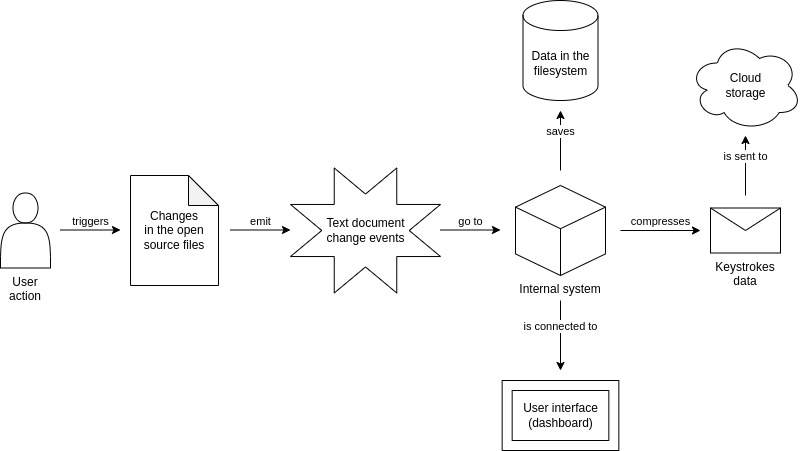
\includegraphics[scale=0.5]{chapters/coding_process_tracker.png}
  \caption{Flow schema of the tool}
\end{figure}

\section{Chosen parts of the tool}

The main component of the internal system are the two buffers filled with the intervals. One of these buffers is the live buffer. The live buffer contains the data gathered lately. It is responsible for creating new intervals from the data that is coming from the user in the real time. The code remembers to save the data in the file system in order to preserve it and not lose it after potential crashes or closing the tool. After saving the data it is possible to remove some intervals from the live buffer in order to be aware of its size and not to allow it to get too big and the memory. The other of the buffers is the static buffer. It is responsible for loading the data from the file system in order for it to be then transferred to the dashboard. The user requests the data from the dashboard.

In order for for the intervals to be visualized they need to be normalized that is made to be of equal lengths. But 0 data you start with the intervals of varying lengths that is of length at most 30 seconds. We need to make them of equivalence and sometimes with that it will equal length being adjustable. Normalization recognizes also that the intervals need to stick to each other however in the Raw data there exist breaks that is there are situations where for some time there is no data start in the file system. So basically we can treat the time spaces that is not covered by the data as intervals with zero keystrokes. Then by interpreting this data such way we can proceed with interpolation let's mention in the figure here. We can imagine that we delete the requested time space into intervals of equal length and then we check if they intersect with the intervals from the real data. The amount of keystrokes that the new interval receives is proportional to the relative size of the intersection to the length of the whole row interval. So it's about you looking at the example from the figure if the intersection constitutes 30\% of the row interval then then we take into account 30\% of keystrokes from this row interval to the new interval of equivalent. The total number of keystrokes associated with this new interval is calculated by summing all of the keystrokes associated with all the intersections from the different row intervals which we can see in the future Maybe we'll delete it later I think.

The user interface constitutes the dashboard that a user can use to view various statistics across different time periods. it is possible through switching modes. The first mode is called the live view.  In this view a user is able to view the latest data. She can also adjust the  time gauge to explore the data in the different time periods (rather in the different lengths from now). The user is provided also with the Calendar view. It is utilized to explore the data from previous days. After selecting today the user can also adjust the time period by using the aforementioned gauges. The parameters of the plot are adjusted automatically in order for the blood to be visible to the user. That means not too convoluted, not too cluttered. The dashboard is connected with the live and static buffers and depending on the View the data is loaded from the light buffer or from the static buffer (that is indirectly from the file system).

\begin{figure}[htbp]
  \centering
  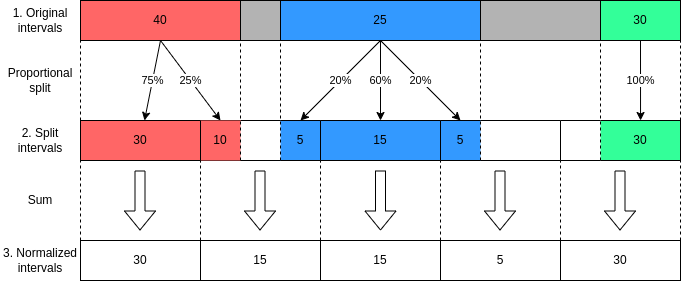
\includegraphics[scale=0.5]{chapters/normalization.png}
  \caption{An intervals normalization example}
\end{figure}

\begin{figure}[htbp]
  \centering
  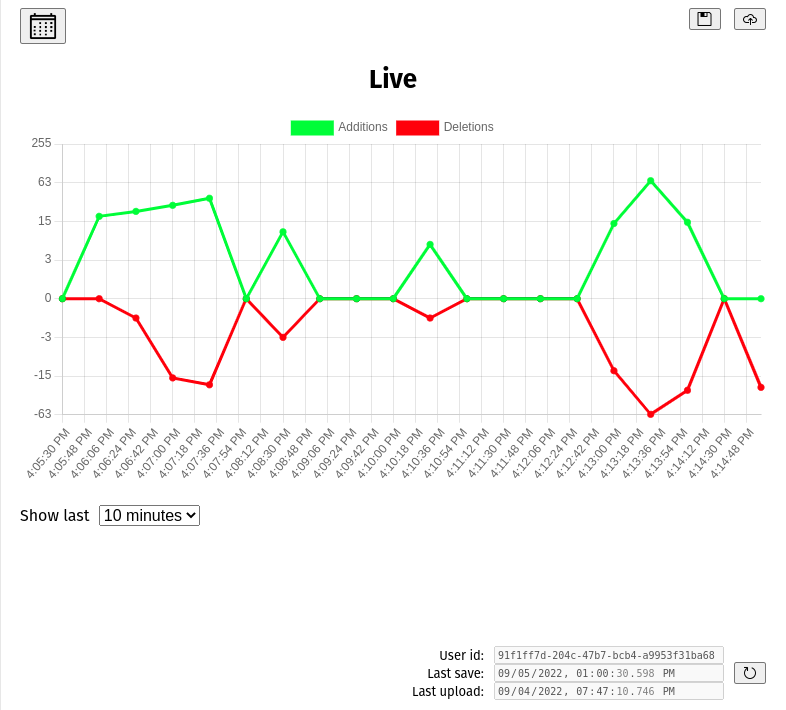
\includegraphics[scale=0.5]{chapters/live-view.png}
  \caption{Live view of the dashboard}
\end{figure}

\begin{figure}[htbp]
  \centering
  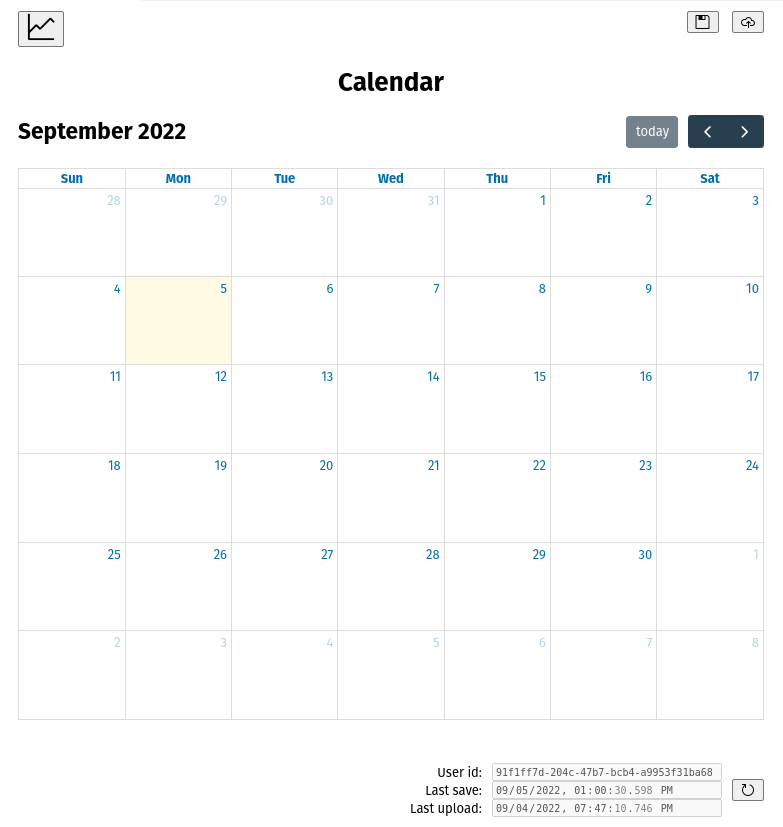
\includegraphics[scale=0.5]{chapters/calendar-view.png}
  \caption{Calendar view of the dashboard}
\end{figure}

\begin{figure}[htbp]
  \centering
  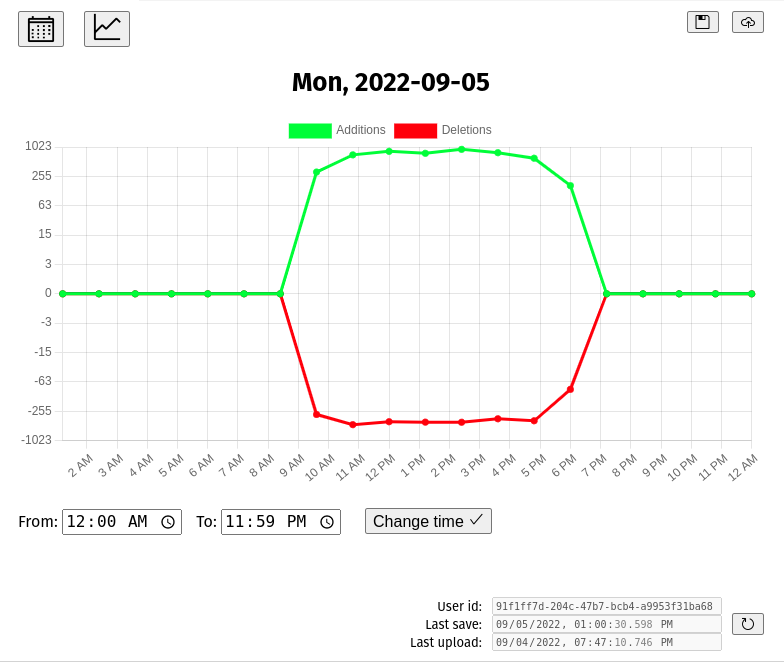
\includegraphics[scale=0.5]{chapters/day-view.png}
  \caption{Day view of the dashboard}
\end{figure}

% TODO file name (not underscore)
\begin{figure}[htbp]
  \centering
  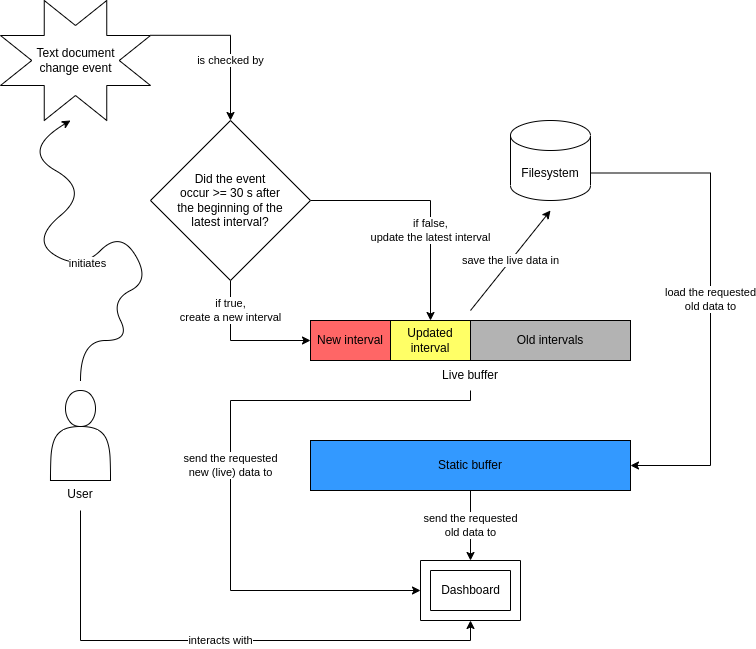
\includegraphics[scale=0.5]{chapters/internal_system.png}
  \caption{Internal system}
\end{figure}

\section{Methods of data analysis}

In the species I will perform a few analytical tests on The Gather the data. This test will include measuring the average length of breaks, their frequency. I will measure the correlations between additions and deletions I will analyze the additions to deletions ratio. I will try as well too observe the existence of morning and evening chronotypes. I will do that bye searching for time periods of particularly increased or decreased activity. I will observe that frequency of extreme points in the plots. This way I can make hypothesis about the actual real actions of programmers because for instance in the Version Control systems merging code may result in high numbers of auditions or deletions. I mean that such suspicious pics of activity May provide evidence to particular actions. Of course I will examine the data also with the with respect to the different programming languages. This way I might find some statistical features that are specific to a particular language.

\chapter{Results}\label{ch:results}

\section{Analysis of data of programmers of different languages}

\chapter{Discussion}\label{ch:discussion}

\section{Revisiting results}

Analysis of the data gathered by the \texttt{MIMUW-MB-TT} plugin sheds some light onto the characteristics of programmers' working day.

Visualizations of a working day of a programmer give potentially valuable insights into the programming process. The developer can introspect and measure his performance. His employer is able to more accurately assess the productivity and potentially provide the assistance where it is needed the most.

Activity analysis shows that understandably most of the work concentrates in the afternoon, but with a notable portion of it done in the evening. Similar patterns emerge when analysing the data from programmers of Python and JS/TS separately. Nevertheless, no sound evidence towards difference of chronotypes between programmers of different languages were discovered.

Breaks analysis unsurprisingly concludes that longer breaks are less frequent that shorter ones and this observation holds for different programming languages and overall. The reason why middle length breaks are more frequent than the shortest ones may just be related to the method of measurement with a break considered as a time space between two data points. Let me remind here that one data point holds information of at most 30 seconds.

Analysis of the ratio of deletions to additions shows that it is more common to add code than to delete it and this trend stays true regardless of the programming language used.

The number of projects per person is observed as at most just a few. Moreover, frequent switching between different projects was not observed.

The data supports the common knowledge that activity dips on weekends. Additionally, it decreases even earlier on Friday which was observed also by Robinson \cite{Rob17LangsUsedAtNight}.

\section{Threats to validity}

\subsection{Doubts about data gathered}

I gathered the data from 15 programmers. This number comes from counting the data packages I have received throughout the study. I assume that each of them comes from a different person, although it is theoretically possible that one person uses the \texttt{MIMUW-MB-TT} plugin on separate workstations, thus is counted multiple times. From my personal talks with the participants, I assess the probability of such occurrences as low.

Although the participants were instructed to use the plugin for at least two weeks, the number of downloads significantly surpass the number of data packages (a minority of them were test downloads by me) and even within the packages there are differences of size between them. Because of that, some participants may influence the final results stronger than the rest.

\subsection{Questions about participants in the study}

Apart from the number of participants, it is important to remember they were not chosen uniformly from the whole community of programmers. Most of them came from the MIMUW faculty as student and it may significantly incluence the final results.

\subsection{\texttt{MIMUW-MB-TT} plugin shortcomings}

Due to the technical obstacles, the plugin does not save the data in the file system right before closing the VS Code window. It just saves the data on 2 minutes interval, so it is possible to lose the data gathered right before closing the IDE.

Additionally, there exist an exploit related to project switching. Since \texttt{workspaceNameHash} relates to the last workspace name recorded for a data point, it is theoretically possible to work within 30 second period on different projects and the system would store such an event as working on just one. This would, however, involve quite a deep knowledge of the plugin and rather unnatural way of typing, so I deem the risk of this exploit influencing the gathered data as minimal.

Apart from that, the plugin allows a situation where \texttt{start} and \texttt{end} are equal for a data point. While this does not constitute a bug by itself, it creates potential confusion and inconvenience when analyzing the gathered data.

\chapter{Conclusions and future work}

% Getting more data
% Publishing the tool

% Say that it's possible to ask why some things happen (annotations)

\chapter{Data and code availability}
In order to streamline my processes and make them more appealing for the public, a part of the agreement was not to publish any keystroke data of my testing subjects. My code is available however at [GitHub]. Anyone also can download my plugin to VSCode at [...].


\appendix

\begin{thebibliography}{99}
\addcontentsline{toc}{chapter}{Bibliography}

\bibitem[1]{Rep02CircadianTiming} Steven M. Reppert, and David R. Weaver. 2002. \textit{Coordination of circadian timing in mammals}. Nature 418, 935–941, doi: \href{https://doi.org/10.1038/nature00965}{10.1038/nature00965}.

\bibitem[2]{Roe03Chronotypes} Till Roenneberg, Anna Wirz-Justice, and Martha Merrow. 2003. \textit{Life between Clocks: Daily Temporal Patterns of Human Chronotypes}. Journal of Biological Rhythms, 18(1), pp. 80–90, doi: \href{https://doi.org/10.1177/0748730402239679}{10.1177/0748730402239679}.

\bibitem[3]{Sto21ProgrammersDo} Dale Stokdyk. 2021. \textit{What Do Programmers Do, Anyway?} Southern New Hampshire University, url: \url{https://www.snhu.edu/about-us/newsroom/stem/what-do-programmers-do}.

\bibitem[4]{Fed21TimeTracking} Tony Fedorenko. 2021. \textit{Time Tracking in Software Development}. Mad Devs, url: \url{https://maddevs.io/customer-university/time-tracking-in-software-development/}.

\bibitem[5]{Gro21SDMHistory} Growin. 2021. \textit{A Brief History of Software Development Methodologies}. Growin Blog, url: \url{https://www.growin.com/blog/history-of-software-development-methodologies/}.

\bibitem[6]{Tho05} Richard C. Thomas, Amela Karahasanovic, and Gregor E. Kennedy. 2005. \textit{An investigation into keystroke latency metrics as an indicator of programming performance}. Proceedings of the 7th Australasian conference on Computing education - Volume 42 (ACE '05). Australian Computer Society, Inc., AUS, 127–134, doi: \href{https://dl.acm.org/doi/10.5555/1082424.1082440}{10.5555/1082424.1082440}.

\bibitem[7]{Lei16} Juho Leinonen, Krista Longi, Arto Klami, and Arto Vihavainen. 2016. \textit{Automatic Inference of Programming Performance and Experience from Typing Patterns}. Proceedings of the 47th ACM Technical Symposium on Computing Science Education (SIGCSE '16). Association for Computing Machinery, New York, NY, USA, 132–137, doi: \href{https://doi.org/10.1145/2839509.2844612}{10.1145/2839509.2844612}.

% \bibitem[8]{}

\bibitem[9]{Lei19Dissertation} Juho Leinonen. \textit{Keystroke Data in Programming Courses}. Ph.D. Dissertation, University of Helsinki, 2019

% \bibitem[10]{}

\bibitem[11]{Zav21MorningEvening} Albina Zavgorodniaia, Raj Shrestha, Juho Leinonen, Arto Hellas, and John Edwards. \textit{Morning or Evening? An Examination of Circadian Rhythms of CS1 Students}. 2021 IEEE/ACM 43rd International Conference on Software Engineering: Software Engineering Education and Training (ICSE-SEET), 2021, pp. 261-272, doi: \href{https://doi.org/10.1109/ICSE-SEET52601.2021.00036}{10.1109/ICSE-SEET52601.2021.00036}.

\bibitem[12]{Fei22DeveloperNames} Dror G. Feitelson, Ayelet Mizrahi, Nofar Noy, Aviad Ben Shabat, Or Eliyahu, and Roy Sheffer. \textit{How Developers Choose Names}. IEEE Transactions on Software Engineering, vol. 48, no. 1, pp. 37-52, 1 Jan. 2022, doi: \href{https://doi.org/10.1109/TSE.2020.2976920}{10.1109/TSE.2020.2976920}.

\bibitem[13]{Mat13PPV} Yoshiaki Matsuzawa, Ken Okada, and Sanshiro Sakai. 2013. \textit{Programming process visualizer: a proposal of the tool for students to observe their programming process}. Proceedings of the 18th ACM conference on Innovation and technology in computer science education (ITiCSE '13). Association for Computing Machinery, New York, NY, USA, 46–51, doi: \href{https://doi.org/10.1145/2462476.2462493}{10.1145/2462476.2462493}.

\bibitem[14]{Bie07FASTDash} Jacob T. Biehl, Mary Czerwinski, Greg Smith, and George G. Robertson. 2007. \textit{FASTDash: a visual dashboard for fostering awareness in software teams}. Proceedings of the SIGCHI Conference on Human Factors in Computing Systems (CHI '07). Association for Computing Machinery, New York, NY, USA, 1313–1322, doi: \href{https://doi.org/10.1145/1240624.1240823}{10.1145/1240624.1240823}.

\bibitem[15]{Lyu21TaskTracker} Elena Lyulina, Anastasiia Birillo, Vladimir Kovalenko, and Timofey Bryksin. 2021. \textit{TaskTracker-tool: A Toolkit for Tracking of Code Snapshots and Activity Data During Solution of Programming Tasks}. Proceedings of the 52nd ACM Technical Symposium on Computer Science Education (SIGCSE '21). Association for Computing Machinery, New York, NY, USA, 495–501, doi: \href{https://doi.org/10.1145/3408877.3432534}{10.1145/3408877.3432534}.

\bibitem[16]{Shr22CodeProcess} Raj Shrestha, Juho Leinonen, Arto Hellas, Petri Ihantola, and John Edwards. 2022. \textit{CodeProcess Charts: Visualizing the Process of Writing Code}. Australasian Computing Education Conference. Association for Computing Machinery, New York, NY, USA, 46–55, doi: \href{https://doi.org/10.1145/3511861.3511867}{10.1145/3511861.3511867}.

\bibitem[17]{Bal13SnapViz} Evan Balzuweit, and Jaime Spacco. 2013. \textit{SnapViz: visualizing programming assignment snapshots}. Proceedings of the 18th ACM conference on Innovation and technology in computer science education (ITiCSE '13). Association for Computing Machinery, New York, NY, USA, 350, doi: \href{https://doi.org/10.1145/2462476.2465615}{10.1145/2462476.2465615}.

\bibitem[18]{Nor08ClockIt} Cindy Norris, Frank Barry, James B. Fenwick Jr., Kathryn Reid, and Josh Rountree. 2008. \textit{ClockIt: collecting quantitative data on how beginning software developers really work}. Proceedings of the 13th annual conference on Innovation and technology in computer science education (ITiCSE '08). Association for Computing Machinery, New York, NY, USA, 37–41, doi: \href{https://doi.org/10.1145/1384271.1384284}{10.1145/1384271.1384284}.

\bibitem[19]{Cla18NightWeekend} Maëlick Claes, Mika V. Mäntylä, Miikka Kuutila, and Bram Adams. 2018. \textit{Do programmers work at night or during the weekend?} Proceedings of the 40th International Conference on Software Engineering (ICSE '18). Association for Computing Machinery, New York, NY, USA, 705–715, doi: \href{https://doi.org/10.1145/3180155.3180193}{10.1145/3180155.3180193}.

\bibitem[20]{Rob17LangsUsedAtNight} David Robinson. 2017. \textit{What Programming Languages Are Used Late at Night?} Stack Overflow Blog, url: \url{https://stackoverflow.blog/2017/04/19/programming-languages-used-late-night/}.

\bibitem[21]{Sil17LangsUsedOnWeekends} Julia Silge. 2017. \textit{What Programming Languages Are Used Most on Weekends?} Stack Overflow Blog, url: \url{https://stackoverflow.blog/2017/02/07/what-programming-languages-weekends/}.

\bibitem[22]{Nov13SEV} Renato Lima Novais, André Torres, Thiago Souto Mendes, Manoel Mendonça, and Nico Zazworka. 2013. \textit{Software evolution visualization: A systematic mapping study}. Information and Software Technology, Volume 55, Issue 11, 2013, Pages 1860-1883, ISSN 0950-5849, doi: \href{https://doi.org/10.1016/j.infsof.2013.05.008}{10.1016/j.infsof.2013.05.008}.

\bibitem[23]{Mat16SoftwareVisualizationReview} Anna-Liisa Mattila, Petri Ihantola, Terhi Kilamo, Antti Luoto, Mikko Nurminen, and Heli Väätäjä. 2016. \textit{Software visualization today: systematic literature review}. Proceedings of the 20th International Academic Mindtrek Conference (AcademicMindtrek '16). Association for Computing Machinery, New York, NY, USA, 262–271, doi: \href{https://doi.org/10.1145/2994310.2994327}{10.1145/2994310.2994327}.

\bibitem[24]{Vih14CodeSnapshotGranularity} Arto Vihavainen, Matti Luukkainen, and Petri Ihantola. 2014. \textit{Analysis of source code snapshot granularity levels}. Proceedings of the 15th Annual Conference on Information technology education (SIGITE '14). Association for Computing Machinery, New York, NY, USA, 21–26, doi: \href{https://doi.org/10.1145/2656450.2656473}{10.1145/2656450.2656473}.

\bibitem[25]{Jad06NoviceCompilationBehaviour} Matthew C. Jadud. 2006. \textit{Methods and tools for exploring novice compilation behaviour}. Proceedings of the second international workshop on Computing education research (ICER '06). Association for Computing Machinery, New York, NY, USA, 73–84, doi: \href{https://doi.org/10.1145/1151588.1151600}{10.1145/1151588.1151600}.

\bibitem[26]{Hum96PSS} Watts S. Humphrey. 1996. \textit{Using a defined and measured Personal Software Process}. IEEE Software, vol. 13, no. 3, pp. 77-88, May 1996, doi: \href{https://doi.org/10.1109/52.493023}{10.1109/52.493023}.

\bibitem[27]{DieSoftViz} Stephan Diehl. 2007. \textit{Software visualization: visualizing the structure, behaviour, and evolution of software}. Springer Science \& Business Media, isbn: 978-3-540-46505-8, doi: \href{https://doi.org/10.1007/978-3-540-46505-8}{10.1007/978-3-540-46505-8}.

\bibitem[28]{Con92SDM} Danny T. Connors. 1992. \textit{Software development methodologies and traditional and modern information systems}. SIGSOFT Softw. Eng. Notes 17, 2 (April 1992), 43–49, doi: \href{https://doi.org/10.1145/130840.130843}{10.1145/130840.130843}.

\bibitem[29]{Put19FourChronotypes} Arcady A. Putilov, Nele Marcoen, Daniel Neu, Nathalie Pattyn, and Olivier Mairesse. 2019. \textit{There is more to chronotypes than evening and morning types: Results of a large-scale community survey provide evidence for high prevalence of two further types}. Personality and Individual Differences, Volume 148, 2019, Pages 77-84, ISSN 0191-8869, doi: \href{https://doi.org/10.1016/j.paid.2019.05.017}{10.1016/j.paid.2019.05.017}.

\bibitem[30]{StackOverflow22Survey} Stack Exchange Inc. 2022. \textit{2022 Developer Survey}. Stack Overflow, url: \url{https://survey.stackoverflow.co/2022/}.

\bibitem[31]{Coh19AltruisticSurvey} Andrew J. Cohen, Sam Washington, Christi Butler, Puneet Kamal, German Patino, Anas Tresh, Jorge Mena, Medina Ndoye, and Benjamin N. Breyer. 2019. \textit{Altruistic donation to improve survey responses: a global randomized trial}. BMC Res Notes, 28 Feb 2019, 12(1):113, doi: \href{https://doi.org/10.1186/s13104-019-4146-y}{10.1186/s13104-019-4146-y}, pmid: 30819217, pmcid: PMC6396474.

\bibitem[32]{Bru11DifferentMotivations} Elisabeth Brüggen, Martin Wetzels, Ko De Ruyter, and Niels Schillewaert. 2011. \textit{Individual Differences in Motivation to Participate in Online Panels: The Effect on Response Rate and Response Quality Perceptions}. International Journal of Market Research, 2011, 369-390, 53, 3, doi: \href{https://doi.org/10.2501/IJMR-53-3-369-390}{10.2501/IJMR-53-3-369-390}.

\bibitem[33]{NIST02SHS} U.S. Department of Commerce and National Institute of Standards and Technology. 2012. \textit{Secure Hash Standard - SHS: Federal Information Processing Standards Publication 180-4}. CreateSpace Independent Publishing Platform, North Charleston, SC, USA, isbn: 978-1-4781-7807-1, doi: \href{https://dl.acm.org/doi/book/10.5555/2408113}{book/10.5555/2408113}.

\bibitem[34]{Lei17PreventIdentification} Juho Leinonen, Petri Ihantola, and Arto Hellas. 2017. \textit{Preventing Keystroke Based Identification in Open Data Sets}. Proceedings of the Fourth (2017) ACM Conference on Learning @ Scale (L@S '17), Association for Computing Machinery, New York, NY, USA, 101–109, doi: \href{https://doi.org/10.1145/3051457.3051458}{10.1145/3051457.3051458}.

\bibitem[35]{Forbes22Philanthropy} Karla D’Alleva Valas. 2022. \textit{3 Trends Shaping Philanthropy In 2022}. Forbes, url: \url{https://www.forbes.com/sites/karladallevavalas/2022/03/31/3-trends-shaping-philanthropy-in-2022/}.

\bibitem[36]{OpenAIGPT3} Adam Rhodes. 2022. \textit{When should you use Files and Documents?}. OpenAI, url: \url{https://help.openai.com/en/articles/5423507-when-should-you-use-files-and-documents}.

\bibitem[37]{JSONLines} Ian Ward. 2022. \textit{JSON Lines Documentation Main Page}. JSON Lines, url: \url{https://jsonlines.org/}.

\bibitem[38]{EULA} Linux Foundation. 2006. \textit{EULA Definition}. The Linux Information Project (LINFO), url: \url{http://www.linfo.org/eula.html}.

\bibitem[39]{VSCodeAPI} Microsoft. 2022. \textit{VS Code API}. Visual Studio Code, url: \url{https://code.visualstudio.com/api/references/vscode-api}.

\bibitem[40]{Nar08DeAnon} Arvind Narayanan, and Vitaly Shmatikov. 2008. \textit{Robust De-anonymization of Large Sparse Datasets}. Proceedings of the 2008 IEEE Symposium on Security and Privacy (SP '08). IEEE Computer Society, USA, 111–125, doi: \href{https://doi.org/10.1109/SP.2008.33}{10.1109/SP.2008.33}.

\bibitem[41]{Hie22Overemployment} Julia Hiemer. 2022. \textit{Between desirability and reality : conceptualization, measurement, causes, and consequences of overemployment}. University of Bamberg Press, doi: \href{https://doi.org/10.20378/irb-53565}{10.20378/irb-53565}.

\bibitem[42]{Luf21BBCOveremployment} Bryan Lufkin. 2021. \textit{The 'overemployed' workers juggling remote jobs}. BBC, url: \url{https://www.bbc.com/worklife/article/20210927-the-overemployed-workers-juggling-remote-jobs}.

\bibitem[43]{Tan11DARPABallons} John C. Tang, Manuel Cebrian, Nicklaus A. Giacobe, Hyun-Woo Kim, Taemie Kim, and Douglas "Beaker" Wickert. 2011. \textit{Reflecting on the DARPA Red Balloon Challenge}. Communications of the ACM, 54, 4 (April 2011), 78–85, doi: \href{https://doi.org/10.1145/1924421.1924441}{10.1145/1924421.1924441}.

\bibitem[44]{Sni15IDEUsageData} Will Snipes, Emerson Murphy-Hill, Thomas Fritz, Mohsen Vakilian, Kostadin Damevski, Anil R. Nair, and David Shepherd. 2015. \textit{A Practical Guide to Analyzing IDE Usage Data}. The Art and Science of Analyzing Software Data, Morgan Kaufmann (2015), 5, 85-138, isbn: 9780124115194, doi: \href{https://doi.org/10.1016/B978-0-12-411519-4.00005-7}{10.1016/B978-0-12-411519-4.00005-7}.

\bibitem[45]{Pro18IDEDataset} Sebastian Proksch, Sven Amann, and Sarah Nadi. 2018. \textit{Enriched event streams: a general dataset for empirical studies on in-IDE activities of software developers}. Proceedings of the 15th International Conference on Mining Software Repositories (MSR '18). Association for Computing Machinery, New York, NY, USA, 62–65, doi: \href{https://doi.org/10.1145/3196398.3196400}{10.1145/3196398.3196400}.

\bibitem[46]{Ama16FeedBag} Sven Amann, Sebastian Proksch, and Sarah Nadi. 2016. \textit{FeedBaG: An interaction tracker for Visual Studio}. IEEE 24th International Conference on Program Comprehension (ICPC), 2016, pp. 1-3, doi: \href{https://doi.org/10.1109/ICPC.2016.7503741}{10.1109/ICPC.2016.7503741}.

\end{thebibliography}


\end{document}


%%% Local Variables:
%%% mode: latex
%%% TeX-master: t
%%% coding: latin-2
%%% End:
